\section{Db2 Graph}
\label{chap:db2graph}

Im Rahmen dieses Kapitels wird IBM Db2 Graph genauer erläutert. Dabei wird der Ansatz, der Aufbau, die Funktionsweise und die bereits bekannten Einschränkungen der von Db2 Graph erläutert. 

\subsection{Ansatz}
\label{db2graph:ansatz}
Db2 Graph wurde mit dem Ziel entwickelt, Informationen mittels Graph-Queries aus einer relationalen Db2 Datenbank abfragen zu können. So wurde Db2 Graph als eine Art Graph-Erweiterung für Db2 konzipiert. Der Einsatz von Db2 Graph setzt folglich eine aktive Instanz von Db2 voraus \cite{vldb_tian, sigmod_tian}. Diese hält hierbei die Informationen, auf die Db2 Graph Zugriff hat, in relationaler Form \cite{vldb_tian, sigmod_tian}. Dabei müssen die Daten nicht für die Einbindung in Db2 Graph angepasst oder umformatiert werden \cite{vldb_tian, sigmod_tian}.

\begin{figure}[h]
    \centering
    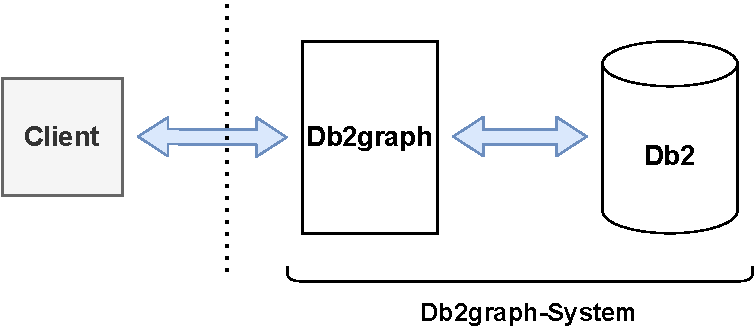
\includegraphics[width=\textwidth]{images/db2graph_system.pdf}
    \vspace{0.1em}
    \caption{Struktur Db2 Graph-System}
    \label{fig:db2graph_system}
\end{figure}

Wie in \autoref{fig:db2graph_system} erkennbar, fungiert Db2 Graph aus architektonischer Sicht als eine Art Proxy-Anwendung für Db2. Dabei übersetzt sie die von einem Client gesendeten Gremlin-Graph-Queries in SQL-An\-wei\-sung\-en und leitet diese anschließend an eine Db2 Instanz weiter \cite{vldb_tian, sigmod_tian}. Darüber hinaus können Db2 und Db2 Graph zusammengefasst als eine Art Hybrides Datenbankmanagementsystem betrachtet werden. Da es Elemente von Graph- und relationalen Datenbanksystemen vereint. So ist es möglich Graph-Anfragen an ein solches System zu stellen, während dem die Daten in relationaler Form gespeichert werden \cite{vldb_tian, sigmod_tian}. Im weiteren Verlauf der Arbeit wird die Kombination aus Db2 und Db2 Graph verkürzt als Db2 Graph-System bezeichnet, wie bereits in \autoref{fig:db2graph_system} dargestellt. 

\subsection{Aufbau}
Wie in \autoref{fig:db2graph_aufbau} beschrieben, handelt es sich bei Db2 Graph um eine modular aufgebaute Anwendung. Die Anwendung besteht dabei aus fünf größeren Komponenten. Die fünf Komponenten übernehmen dabei die folgenden Rollen und Aufgaben: 

\begin{itemize}
    \item \textbf{TinkerPop-Stack}\\Stellt das Grundgerüst für Db2 Graph dar. Er parst eingehende Gremlin-Queries und erstellt auf Basis dessen einen Query-Plan bzw. Abfrage-Plan \cite{vldb_tian}. Dabei interagiert er über API-Aufrufe mit den anderen Modulen \cite{vldb_tian}.
    \item \textbf{Topology}\\Beinhaltet die Funktionalität für das Mapping von relationalen Tabellen auf eine Graph-Struktur \cite{vldb_tian, sigmod_tian}.
    \item \textbf{Graph Structure}\\Hierbei handelt es sich um eine eigene Implementierung einer Graph-Struktur, auf deren Basis TinkerPop arbeitet \cite{vldb_tian}. Eine Implementierung dieser Struktur wird benötigt, um den vom TinkerPop-Stack erstellten Query-Plan durchzuführen \cite{sigmod_tian}. 
    \item \textbf{SQL-Dialect}\\Diese Komponente stellt die Funktionalität für die Erzeugung von Db2-kompatiblen SQL-Anweisungen bereit \cite{sigmod_tian}.
    \item \textbf{Traversal-Strategy}\\Dieses Modul stellt dem TinkerPop-Stack optimierte Traversal-Strategies zur Verfügung. Diese werden eingesetzt, um einen vom TinkerPop-Stack aufgestellten Query-Plan zu optimieren, bevor dieser ausgeführt wird \cite{sigmod_tian}.  
\end{itemize}

So stellt also der TinkerPop-Stack den Kern von Db2 Graph dar. Die Topology-, Graph-Structure- und SQL-Dialect-Komponente hingegen bieten Db2 Graph und Db2 spezifische Funktionalität, auf die der TinkerPop-Stack zugreifen kann. Das Traversal-Strategy-Modul stellt darüber hinaus dem TinkerPop-Stack, optimierte Traversal-Strategies zur Verfügung. Diese helfen dem TinkerPop-Stack dabei die Performance von Query-Plans zu verbessern.  

\begin{figure}[h]
    \centering
    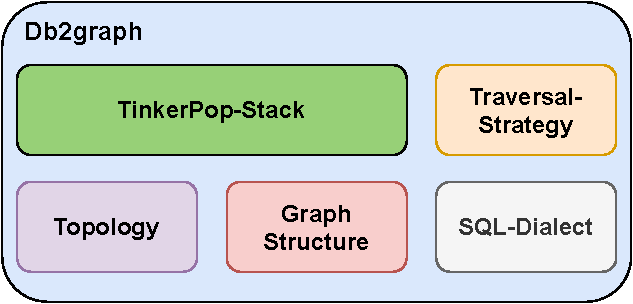
\includegraphics[width=\textwidth]{images/db2graph_components.pdf}
    \caption{Aufbau von Db2 Graph}
    \label{fig:db2graph_aufbau}
    \vspace{0.5em}
    \textit{Der hier gezeigter Aufbau von Db2 Graph   orientiert sich an der Beschreibung der System-Architektur in \cite{vldb_tian} und \cite{sigmod_tian}.}
\end{figure}

\subsection{Funktionsweise}
\label{db2graph:funktionsweise}
Um die Funktionsweise von Db2 Graph genauer zu erläutern, wird in diesem Abschnitt die Funktionsweise aus verschiedenen Perspektiven erläutert. Im Rahmen der ersten externen Perspektive wird detailliert darauf eingegangen, wie ein Db2 Graph-System die Anfrage eines Clients verarbeitet. Dabei wird erläutert, wie die Verarbeitung einer Gremlin-Query im Kontext einer Client-Anwendung, Db2 Graph und Db2 erfolgt. Bei der zweiten Perspektive handelt es sich hingegen um die Db2 Graph interne Perspektive. Im Zuge dessen wird beschrieben, wie eine Gremlin-Abfrage von einer Db2 Graph-Anwendung intern verarbeitet wird. Im Anschluss an diese beiden Perspektiven wird der Begriff und die Funktionsweise des Mapping in Db2 Graph genauer erläutert.

\subsubsection{Extern}
Die Funktionsweise beziehungsweise der Ablauf der Verarbeitung einer Graph-Query im Kontext eines Clients und Db2 Graph-Systems läuft wie folgt ab:

\begin{enumerate}
    \item Ein Client sendet eine Gremlin-Query an Db2 Graph. 
    \item Db2 Graph wandelt die Gremlin-Query in SQL-Statements um. 
    \item Db2 Graph sendet die erzeugten SQL-Statements an Db2.
    \item Db2 verarbeitet die SQL-Statements.
    \item Db2 leitet die Ergebnisse an Db2 Graph weiter.
    \item Db2 Graph bereitet die von Db2 empfangen Ergebnisse für den Client auf. 
    \item Db2 Graph übermittelt die Ergebnisse an den Client.
\end{enumerate}

Die soeben beschrieben Schritte des Ablaufs können dabei den in der \autoref{fig:db2graph_processing} aufgeführten Schritten zu geordnet werden. Die in \autoref{fig:db2graph_processing} als grün gekennzeichnet Pfeile markieren dabei die Schritte, in den die Anfrage in Form einer Gremlin-Query oder SQL-Anfragen weitergeleitet oder verarbeitet wird. Die Pfeile, welche in \autoref{fig:db2graph_processing} lila gefärbt sind, heben die Schritte hervor, in denen die abgefragten Daten transformiert oder weitergeleitet werden.

\begin{figure}[h]
    \centering
    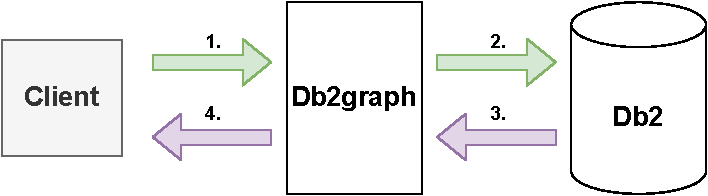
\includegraphics[width=\textwidth]{images/db2graph_processing.pdf}
    \caption{Externe Verarbeitung Db2 Graph}
    \label{fig:db2graph_processing}
    \vspace{1em}
    \textit{Die hier dargestellten Abläufe basieren hierbei unter anderem auf den in \cite{vldb_tian} und \cite{sigmod_tian} beschrieben Abläufen der Verarbeitung. Darüber hinaus wurden auch einige kleinere Details von \cite{tinkerpop_2020} bezogen.} 
\end{figure}

\subsubsection{Intern}
Im Rahmen dieses Unterabschnitts wird dargelegt, wie eine von Db2 Graph empfangene Gremlin-Query intern verarbeitet wird. Der Ablauf kann dabei in die folgenden Schritte gegliedert werden: 

\begin{enumerate}
    \item Ein Client baut Verbindung auf und sendet eine Gremlin-Query Db2 Graph.
    \item Der TinkerPop-Stack lädt Informationen über die Beschaffenheit des in der Gremlin-Query enthaltenen Zielgraphen aus Topology-Komponente \cite{vldb_tian,sigmod_tian, yt_tian}.
    \item Der TinkerPop-Stack erstellt auf Basis der Gremlin-Query und der Topologie-Informationen einen logischen Query-Plan auf \cite{vldb_tian,sigmod_tian, yt_tian}. 
    \item Der TinkerPop-Stack nutzt das Traversal-Strategy-Modul, um den logischen Query-Plan zu optimieren \cite{vldb_tian,sigmod_tian, yt_tian}.
    \item Der TinkerPop-Stack wandelt den optimierten logischen Query-Plan in einen physikalischen Query-Plan um \cite{vldb_tian,sigmod_tian, yt_tian}. 
    \item Bei der Ausführung der Steps im physikalischen Query-Plan werden API-Zugriffe auf die Graph-Structure-Komponente durchgeführt. Um die für diese Zugriffe benötigten Informationen zu beschaffen, lädt die Graph-Structure-Komponente Informationen aus dem Topology-Modul und nutzt die SQL-Dialect-Komponente für die Erzeugung von SQL-Statements. \cite{vldb_tian,sigmod_tian, yt_tian} 
    \item Die von der Graph-Structure-Komponente erzeugten SQL-Statements werden an eine Db2 Instanz gesendet und von dieser verarbeitet. \cite{vldb_tian,sigmod_tian, yt_tian}
    \item Die daraufhin von Db2 erhalten und zurückgesendeten Ergebnisse werden von der Graph-Structure-Komponente verarbeitet. \cite{yt_tian} 
    \item Die Graph-Komponente nutzt die verarbeiteten Ergebnisse, um die API-Aufrufe des TinkerPop-Stacks zu beantworten. \cite{vldb_tian,sigmod_tian, yt_tian} 
    \item Nach der Durchführung des physikalischen Query-Plans -- inklusive der API-Aufrufe auf die Graph-Structure-Komponente -- werden die Ergebnisse vom TinkerPop-Stack an den Client übermittelt \cite{vldb_tian,sigmod_tian, yt_tian}.
\end{enumerate}

Die in der zuvor aufgelisteten Schritten werden im Fall von 1. bis 7. auch nochmal in der \autoref{fig:db2graph_intern_processing} visuell dargestellt.

\begin{figure}[h]
    \centering
    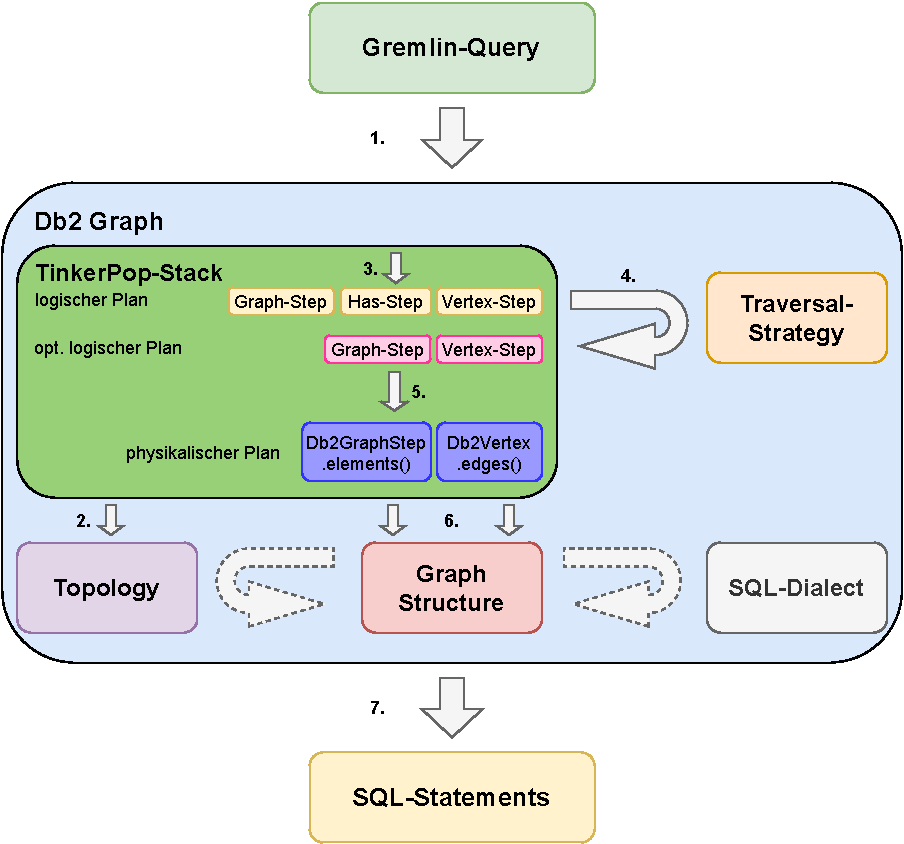
\includegraphics[width=\textwidth]{images/db2graph_intern_processing.pdf}
    \caption{Interne Verarbeitung Db2 Graph}
    \label{fig:db2graph_intern_processing}
    \vspace{1em}
    \textit{Die in der Abbildung dargestellten Abläufe basieren auf den in \cite{yt_tian}, \cite{vldb_tian} und \cite{sigmod_tian} beschrieben Abläufen.} 
\end{figure}

\subsubsection{Mapping}
Bei dem sogenannten Mapping handelt es sich um den Db2 Graph-internen Prozess beziehungsweise Technik, bei dem eine Graph-Struktur relationalen Daten überge\-stülpt wird beziehungsweise diese überlagert. Der Prozess kann auch als Graph-Overlaying bezeichnet werden. Im weiteren Rahmen der Arbeit wird der Prozess aber der Einfachheit halber als Mapping bezeichnet. Denn im Kern handelt es sich hierbei um ein Mapping von relationalen Tabellen und Spalten auf Graph-Elemente, wie Knoten und Kanten. Für die Bereitstellung und Verarbeitung des Mapping in Db2 Graph ist dabei die Topology-Komponente zuständig. 

Um das Mapping von relationalen auf Graph-Strukturen durchzuführen, werden den relationalen Tabellen verschiedene Rollen zugewiesen. Dabei sind die zwei folgenden Rollen verfügbar:
\begin{itemize}
    \item \textbf{VertexTable}\\Die Zeilen einer Tabelle werden als Knoten auf einen Graph gemappt \cite{sigmod_tian, yt_tian}.
    \item \textbf{EdgeTable}\\Die Zeilen dieser Tabelle werden als Kanten auf einen Graph gemappt \cite{sigmod_tian, yt_tian}.
\end{itemize}

Um Verbindungen zwischen Kanten und Knoten herzustellen  verfügt eine VertexTable über eine \texttt{vid}. Diese \texttt{vid} kann als eine Art Primärschlüssel betrachtet werden. Die \texttt{vid} setzt sich dabei aus einer oder mehreren Spalten einer relationalen Tabelle und einem Prefix zusammen \cite{sigmod_tian, yt_tian}, siehe \texttt{prefix} und \texttt{id\_cols} Zeile 5-6 in \autoref{src:mapping_example}. Ihr Zweck ist es dabei, immer einen einzigen bestimmten Knoten über den Wert den \texttt{vid} identifizieren zu können \cite{sigmod_tian, yt_tian}. 

Auf Basis dieser \texttt{vid} -- Zeile 4-7 \autoref{src:mapping_example} –– setzt beim Mapping auch die EdgeTable auf. Um einen Quell- und Ziel-Knoten für eine Kante festzulegen, wird bei den EdgeTables angegeben, welche Spalten der Tabelle einen jeweiligen Quell- und Ziel-Knoten referenzieren, siehe \texttt{src\_v\_cols} und \texttt{dst\_v\_cols} in Zeile 21 und 22 des \autoref{src:mapping_example}. Dabei muss, um einen Verstoß gegen die referenzielle Integrität zu vermeiden, der Wert der \texttt{vid} dem Wert der referenzierten Spalten in der EdgeTable entsprechen. Darüber hinaus muss festgelegt werden, wie die \texttt{table\_id} der VertexTables lauten, die den Quell- und Ziel-Knoten einer Kante beinhalten, siehe die Zeilen 8, 23 und 24 in \autoref{src:mapping_example}. Durch diese Verweise und Referenzierung wird in der Konfiguration ein Mapping definiert, welches die Topologie eines Graphen bestimmt. 

Wie im \autoref{src:mapping_example} erkennbar lässt die Konfiguration auch weitere Anpassungen bezüglich des Mappings und der Graph-Topologie zu. So ist es beispielsweise möglich die Labels für Knoten und Kanten auf Basis einer VertexTable oder EdgeTable zu definieren, siehe Zeile 15 und 43 \autoref{src:mapping_example}. Der Kern des Mappings spielt sich dabei aber wie zuvor beschrieben auf Basis der Parameter \texttt{vid}, \texttt{table\_id}, \texttt{src\_v\_cols}, \texttt{dst\_v\_cols} sowie \texttt{dst\_v\_tables} und \texttt{src\_v\_tables} ab. Diese Werte bestimmten, wie die relationalen Daten auf einen Graph abgebildet werden.

\begin{lstlisting}[caption={Beispiel Auschnitt Mapping Konfiguration},language=json,label=src:mapping_example]
{
    "v_tables": [
            {
            "vid": {
                "prefix": "LINKDB0.NODETABLE",
                "id_cols": ["ID"]
            },
            "table_id": "LINKDB0.NODETABLE",
            "table": {
                "schema_name": "LINKDB0",
                "table_name": "NODETABLE"
            },
            "label": {
                "fixed_label": true,
                "label": "NODETABLE"
            }
        }
    ],
    "e_tables": [
        {
            "src_v_cols": ["ID1"],
            "dst_v_cols": ["ID2"],
            "src_v_tables": ["LINKDB0.NODETABLE"],
            "dst_v_tables": ["LINKDB0.NODETABLE"],
            "eid": {
                "implicit_id": false,
                "id": {
                    "prefix": "LINKDB0.LINKTABLE",
                    "id_cols": [
                        "LINK_TYPE",
                        "ID1",
                        "ID2"
                    ]
                }
            },
            "table_id": "LINKDB0.LINKTABLE",
            "table": {
                "schema_name": "LINKDB0",
                "table_name": "LINKTABLE"
            },
            "label": {
                "fixed_label": true,
                "label": "LINKTABLE"
            }
        }
    ]
}
\end{lstlisting}

Abschließend zum Thema Mapping sollte auch darauf hingewiesen werden, dass nicht alle Tabellen einer Datenbank oder eines bestimmten Schemas auf einen Graphen gemappt werden müssen. Es ist vollkommen legitim relationalen Tabellen keine Rolle als VertexTable oder EdgeTable zuzuweisen, sollten die Daten im Kontext des Graphen nicht benötigt werden. 

\subsection{Fähigkeiten \& Einschränkungen}
Im Rahmen dieses Kapitels werden die bekannten Fähigkeiten und Einschränkungen von Db2 Graph kurz zusammengefasst. Dies ist hier von besonderem Interesse, da es sich bei Db2 Graph in Kombination mit Db2 um eine Art hybrides Datenbankmanagementsystem handelt. Auf die besonderen Eigenschaften des Systems, die sich aus der Verbindung von relationalem und Graph-Datenbanksystem ergeben, wird hier auch ebenfalls eingegangen. 

Db2 Graph verfügt über die folgenden Fähigkeiten und Einschränkungen:

\begin{itemize}
    \item \textbf{Read-Only-Queries}\\
    Db2 Graph verfügt über eine read-only Implementierung von Apache TinkerPop, daher ist es dazu in der Lage nahe zu alle read-only Gremlin-Queries zu verarbeiten \cite{ibm_docs_limitiations}. Umgekehrt bedeutet dies allerdings auch, dass Db2 Graph nicht fähig ist schreibende Gremlin-Queries zu verarbeiten.
    \item \textbf{Optimierung}\\
    Db2 Graph verfügt über mehrere Mechanismen um die Verarbeitung von empfangen Gremlin-Queries zu optimieren, mehr dazu in \autoref{subsec:db2graph_optimierung}.
    \item \textbf{Datentypen}\\
    Von Db2 Graph werden nur Datentypen unterstützt, die auch in Db2 vorhanden sind \cite{ibm_docs_limitiations}. Das bedeutet, das nur diese Datentypen als Property-Type eines Knotens oder einer Kante eingesetzt werden kann \cite{ibm_docs_limitiations}. Somit ist es auch nicht möglich verschachtelte Datentypen -- wie z.B. in Neo4j -- als Property-Type zu nutzen. Schließlich werden diese nicht von Db2 Graph unterstützt.
    \item \textbf{Festes Schema}\\
    Daten die von Db2 Graph abgefragt werden können verfügen über ein festes Schema. Diese ergibt sich daraus, dass die Daten in einer Db2 Instanz (relational) gehalten und gespeichert werden \cite{sigmod_tian,vldb_tian,yt_tian}.
    \item \textbf{Gremlin-Graph-API}\\
    Die Gremlin-Graph-API wird von Db2 Graph nicht unterstützt \cite{ibm_docs_limitiations}. Mehr dazu in !TODO REF Erweiterbarkeit.
\end{itemize}

\subsection{Optimierung}
\label{subsec:db2graph_optimierung}

Im Kontext dieses Abschnitts wird eine Übersicht über die Optimierungsmechanismen von Db2 Graph geben. Dabei stützt sich diese Arbeit, auf die in \cite{sigmod_tian} beschrieben Optimierungstechniken \cite{sigmod_tian}. Auch die Unterteilung der Mechanismen in die Kategorien Data-Independent Optimizations und Data-Dependent Optimizations werden dabei aus \cite{sigmod_tian} übernommen.

\subsubsection{Data-Independent Optimizations}
\label{subsubsec:data_independent_optimizations}
Bei Data-Independent Optimizations handelt es sich um Optimierungstechniken, die Teil des Traversal-Strategy Moduls sind \cite{sigmod_tian}. Sie werden eingesetzt, um einen logischen Query-Plan zu optimieren. Ihr Anwendung erfolgt dann, wenn bestimmte Muster erkannt werden. Optimierungen die in diese Kategorie fallen, können dem Schritt 4. in \autoref{fig:db2graph_intern_processing} zugeordnet werden. 

In die Kategorie Data-Independent Optimizations fallen dabei die folgenden Techniken: 

\begin{itemize}
    \item \textbf{Predicate Pushdown with Filter Steps}\\
    Diese Optimierung wird angewandt, wenn ein Graph-Structure-Access-Step wie \texttt{g.V()} oder \texttt{g.E()} von einem oder mehreren Filter-Steps gefolgt wird \cite{sigmod_tian}. Dabei werden alle Filter-Steps in Graph-Structure-Access-Step als Predicats eingebettet \cite{sigmod_tian}. Das Endprodukt der Optimierung stellt nun ein neuer Graph-Step dar, welcher auf Basis des Graph-Structure-Access-Steps und der Filter-Steps erstellt wurde \cite{sigmod_tian}. 
    
    Um die Funktionsweise der Optimierung zu verdeutlichen, kann die Gremlin-Query \code{g.V().has(``id", 1).has(``type'', ``A'')} herangezogen werden. Bei der Optimierung des aus dieser Query resultierenden Query-Plans, werden der Graph-Structure-Access-Step und die Has-Steps in einen einzigen neuen Graph-Step umgewandelt. So wird bei der Ausführung dieses neuen Graph-Steps der SQL-Code \code{SELECT * FROM VertexTable WHERE id = 1 AND type = ``A''} erzeugt. An diesem lässt sich erkennen, dass die Has-Steps als Teil einer \code{WHERE}-Bedingung in die Abfrage eingebettet wurden.

    Als Resultat dieser Optimierung sendet Db2 Graph somit weniger Anfragen an DB2 und erhält zugleich kleinere Ergebnismengen.

    \item \textbf{Projection Pushdown with Properties Steps}\\
    Diese Optimierung greift, wenn Db2 Graph eine Gremlin-Query verarbeitet, in der bestimmte Properties von Knoten oder Kanten abgefragt werden \cite{sigmod_tian}. Hierbei werden die abgefragten Properties in die Projektion eines vorausgegangenen Gremlin-Steps eingebettet. Auf diese Weise erhält Db2 Graph eine kleinere Ergebnismenge von Db2. Diese umfasst dabei lediglich die benötigten Informationen. Dabei gilt es zu beachten, das neben den angegeben Properties, auch die \texttt{id\_cols} -- siehe Zeile 6 und 28 in \autoref{src:mapping_example} -- als Informationen von Db2 Graph benötigt werden. 

    Ein gutes Beispiel für dafür, wie die Optimierung durchgeführt wird, bietet die Gremlin-Query \code{g.V().values(``data'', ``time'')}. Die Projektion aus dem Values-Step wird dabei zusammen mit den \texttt{id\_cols} in den Graph-Structure-Access-Step integriert. So wird der neue optimierte Graph-Step später in folgende SQL-Anweisungen übersetzt \code{SELECT id, type,
    data, time FROM VertexTable}. Ohne die Optimierung wäre der Graph-Step so übersetzt worden: \code{SELECT * FROM VertexTable}.

    \item \textbf{Aggregate Pushdown with Aggregation Steps}\\
    Wenn ein Graph-Structure-Access-Step von einem Aggregations-Step gefolgt wird, wie \texttt{count}, \texttt{mean}, \texttt{min}, \texttt{max} und \texttt{sum} setzt die Optimierung ein \cite{sigmod_tian}. Dabei wird die Aggregation in den Graph-Structure-Access-Step eingebettet \cite{sigmod_tian}. Dadurch erhält Db2 Graph bei der Ausführung des neuen Graph-Steps ausschließlich die bereits von Db2 aggregierten Ergebnisse.
    
    Die Gremlin-Query \code{g.V().count()} würde dabei zu einem einzelnen Graph-Step optimiert \cite{sigmod_tian}. Dieser ließe sich dann später bei der Ausführung in den SQL-Code \code{SELECT COUNT(*) FROM VertexTable} übersetzen \cite{sigmod_tian}.

    \item \textbf{GraphStep::VertexStep Mutation}\\
    Diese Optimierung wird angewandt, wenn ein Graph-Structure-Access-Step Vertexes abfragt und von einem Vertex-Step \cite{sigmod_tian}. Die Optimierung zielt dabei darauf ab unnötige SQL-Abfragen zu vermeiden \cite{sigmod_tian}. 

    Die Optimierung lässt sich dabei verständlich anhand der Gremlin-Query \code{g.V(ids).outE()} \cite{sigmod_tian}. Bei den \texttt{ids} handelt es sich hierbei um ein Set an \texttt{vids}, wie in Zeile 4 \autoref{src:mapping_example}. Ohne diese Optimierung würden auf Basis der nicht optimierten Graph-Steps die zwei folgenden SQL-Anweisungen generieren: \code{SELECT * FROM VertexTable WHERE id IN (ids)} und \code{SELECT * FROM EdgeTable WHERE src\_v IN (ids)} \cite{sigmod_tian}. Bei genauerer Betrachtung des ersten SQL-Statements fällt auf, dass diese keinen relevanten Beitrag zur Beantwortung der Gremlin-Query leistet \cite{sigmod_tian}. An dieser Stelle setzt die Optimierung an \cite{sigmod_tian}. Sie mutiert den Vertex-Step in einen Graph-Step der Edges abfragt und die \texttt{ids} als Predicats übernimmt \cite{sigmod_tian}. Dadurch wird die obsolete Abfrage eliminiert und lediglich die SQL-Query \code{SELECT * FROM EdgeTable WHERE src\_v IN (ids)} generiert und an Db2 gesendet \cite{sigmod_tian}.

    \item \textbf{Combined Optimizations}\\
    Alle vorausgegangenen Optimierungen können miteinander kombiniert werden, falls nötig \cite{sigmod_tian}. Dies sorgt dafür, dass die Gremlin-Query \code{g.V(ids).outE().has("link\_type", 123456789).count()} .
\end{itemize}

\subsubsection{Data-Dependent Optimizations}

Die sogenannten Data-Dependent Optimizations stellen Optimierungstechniken dar, die auf Basis von Topologie Informationen des Graphen Optimierung vornehm\-en. Diese Optimierungen werden dabei im Rahmen des Graph Structure Moduls zur Laufzeit angewandt. Im vorigen Unterabschnitt \nameref{subsubsec:data_independent_optimizations} wurden hauptsächlich Optimierungen angesprochen, die dazu dienen:
\begin{itemize}
    \item unnötige Abfragen zu vermeiden, 
    \item die Antwortmenge so gering wie nur möglich zu halten und 
    \item das Processing, wenn möglich in Db2 statt Db2 Graph durchzuführen.  
\end{itemize}
Im Gegensatz versuchen die Data-Dependent Optimizations die Menge, auf die eine Abfrage durchgeführt wird so klein wie möglich zu halten. Um dies zu erreichen, werden Topologie Informationen herangezogen.

Die folgenden Optimierungstechniken werden dabei herangezogen:
\begin{itemize}
    \item \textbf{Using Source/Destination Vertex Tables}\\
    Diese Optimierung setzt bei den Source- und Destination-Tabellen an, siehe \texttt{src\_v\_tables} und \texttt{dst\_v\_tables} in Zeile 23 - 24 \autoref{src:mapping_example}. Diese werden zur Laufzeit herangezogen um die Abfrage von allen bzw. überflüssigen Tabellen ausschließen zu können \cite{sigmod_tian}.

    Um die Funktionsweise zu verdeutlichen, kann die Abfrage eines beliebigen ausgehenden Knoten einer Kante herangezogen werden \cite{sigmod_tian}. Diese könnte als Gremlin-Query wie folgt aussehen \code{e.outV()} \cite{sigmod_tian}. Ohne die Anwendung der hier besprochenen Optimierungstechniken, würde die Query in das folgende SQL-Statements übersetzt werden \code{SELECT * FROM VertexTable WHERE dst\_v = e.dst\_v} \cite{sigmod_tian}. Dieses SQL-Statement müsste dann einmal alle bekannten Vertex-Tabellen abfragen \cite{sigmod_tian}. Mit der Optimierung hingegen, kann auf Basis der \texttt{dst\_v\_tables} aus der Topologie eine Untermenge an Vertex-Tabellen identifiziert werden, an die durch eine solche SQL-Abfrage abgefragt werden muss \cite{sigmod_tian}. Somit lässt sich die Menge an die Vertex-Tabellen die abgefragt werden müssen, auf eine kleine notwendige Untermenge beschränken \cite{sigmod_tian}. Vergleichbares ist auch im Zusammenhang mit Source-Tabellen möglich.
    \item \textbf{When A Vertex Table Is Also An Edge Table}
    Diese spezielle Optimierungstechnik kann angewendet werden, wenn eine Vertex-Tabelle und eine Edge-Tabelle auf dieselbe relationale Tabelle in Db2 gemappt werden. Dann besteht die Möglichkeit, dass eine Abfrage komplett eingespart werden kann und abgefragte Daten auf Basis eines  bereits zuvor abgefragten Graph-Struktur, rekonstruiert werden können. 

    Wird wieder das Beispiel der Gremlin-Query \code{e.outV()} herangezogen. So besteht die Möglichkeit, dass wenn die gemappten relationalen Tabellen einer Edge-Tabelle und Vertex-Tabelle einander entsprechen und die definierten Properties und Felder der Edges-Tabelle mit denen der Vertex-Tabelle überschneiden, eine Abfrage des Vertexes aus der Vertex komplett eingespart werden kann.
\end{itemize}

\subsection{Versionen}
